\documentclass[11pt]{article} % use larger type; default would be 10pt

\usepackage[utf8]{inputenc} % set input encoding (not needed with XeLaTeX)

\usepackage{tikz}
\begin{document}

% The coordinate shape is handled in a special way by TikZ. When a node x whose shape is
%  'coordinate' is used as a coordinate (x), this has the same eect as if you had said (x.center).
%  None of the special "line shortening rules" apply in this case. 
%  This can be useful since, normally, the line shortening causes paths to be segmented 
%  and they cannot be used for filling. Here is an example that demonstrates the dierence:

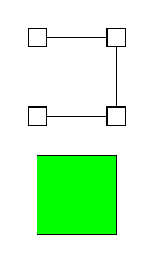
\begin{tikzpicture}[every node/.style={draw}]

% ( Note that yshift separates all coordinates vertically, i.e.
%  both paths are using the same space! )

\path[yshift=1.5cm,shape=rectangle]
(0,0) node(a1){} (1,0) node(a2){}
(1,1) node(a3){} (0,1) node(a4){};
\filldraw[fill=green] (a1) -- (a2) -- (a3) -- (a4);

\path[shape=coordinate]
(0,0) coordinate(b1) (1,0) coordinate(b2)
(1,1) coordinate(b3) (0,1) coordinate(b4);
\filldraw[fill=green] (b1) -- (b2) -- (b3) -- (b4);
\end{tikzpicture}

\end{document}